% Titolo della sezione e label. Vi consiglio, per questioni di ordine mentale e rapidità successiva di reference, di etichettare le label in modo sensato, con riferimento chiaro a cosa si sta etichettando. Quindi sec:nomesezione per una sezione, im:nomeimmagine per una immagine, e via dicendo.
\section{Primo Esercizio}\label{sec:primoEsercizio} 
Amplificatore Audio per Auricolari
\begin{figure}[h]
    \centering
    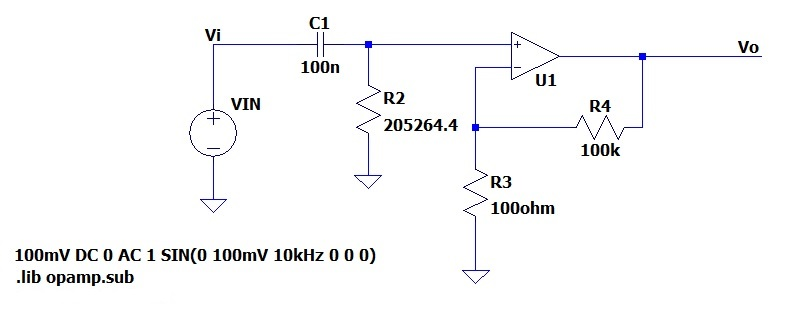
\includegraphics[width=0.9\textwidth]{Figure/Circuito1.jpg}
    \caption{Circuito del primo esercizio}
    \label{fig:Circuito1}
\end{figure}\\
Listato SPICE della rete considerata:\\
\\
C1 N001 Vi 100n\\
R2 N001 0 205264.4\\
R3 N002 0 100\\
R4 Vo N002 100k\\
XU1 N002 N001 Vo opamp Aol=100K GBW=10Meg\\
VIN Vi 0 100mV DC 0 AC 1 SIN(0 100mV 10kHz 0 0 0)\\
.ac dec 10 1 1MEG\\
.lib opamp.sub\\
.backanno\\
.end\\
\subsection{Analisi Analitica}\label{subsec:analisiAnalitica}
Si procede considerando l'amplificatore ideale
\begin{itemize}
\item 
    \begin{equation}\label{eq:eqMorsettiAmplificatore}
    V_{-} = V_{+} = V_{i} \dfrac{R_{2}}{R_{2} + \dfrac{1}{sC_{2}}} = V_{i} \dfrac{sR_{2}C_{2}}{1 + sC_{2}R_{2}}
    \end{equation}
\item 
    \begin{equation}\label{eq:eqCorrenteR3}
    I_{R_{3}} = \dfrac{V_{-}}{R_{3}} = V_{i} \dfrac{sR_{2}C_{2}}{R_{3} (1 + sC_{2}R_{2})}
    \end{equation}
\item
    \begin{equation}\label{eq:eqTensioneUscita1}
    V_{o} = I_{4} R_{4} + V_{-} = V_{i} ( \dfrac{R_{4}}{R_{3}} \dfrac{sR_{2}C_{2}}{1 + sC_{2}R_{2}} + \dfrac{sR_{2}C_{2}}{1 + sC_{2}R_{2}} )
    \end{equation}
    \begin{equation}\label{eq:eqTensioneUscita2}
    V_{o} = V_{i} ( \dfrac{sR_{2}C_{2} (R_{3}+R_{4})}{R_{3}} \dfrac{1}{1 + sC_{2}R_{2}}  )
    \end{equation}
\end{itemize}
La risposta in frequenza del circuito considerato presenta uno zero nell'origine e un polo ad una frequenza f.
\begin{itemize}
\item 
    Guadagno \begin{equation}\label{eq:eqGuadagno}
    K = \dfrac{R_{2}C_{2} (R_{3}+R_{4})}{R_{3}} = 20,547
    \end{equation}
    \begin{equation}\label{eq:eqGuadagnoDecibel}
    (K)_{dB} = 20 log_{10} (K) = 26,25\hspace{2pt}dB
    \end{equation}
\item 
    La risposta presenta uno zero nell'origine
    \begin{equation}\label{eq:eqPoloOrigine}
    +20 \hspace{2pt}\dfrac{dB}{DEC}
    \end{equation}
\item
    La risposta presenta un polo alla frequenza di taglio
    \begin{equation}\label{eq:eqPulsazioneTaglio}
    \omega = \dfrac{1}{R_{2}C_{2}} = 48,71
    \end{equation}
    \begin{equation}\label{eq:eqFrequenzaTaglio}
    f = \dfrac{\omega}{2\pi} = 7,75\hspace{2pt}Hz
    \end{equation}
\end{itemize}

\subsection{Frequenza di Taglio Inferiore}\label{subsec:frequenza_taglio_inferiore}
Come calcolato precedentemente la risposta in frequenza presenta un polo alla frequenza di taglio  (Equazione n° \ref{eq:eqFrequenzaTaglio})
$$f = \dfrac{\omega}{2\pi} = 7,75\hspace{2pt}Hz$$

\subsection{Diagramma di Bode}\label{subsec:diagramma_bode}
Il diagramma di Bode che risulta dall'analisi analitica è il seguente\\
\begin{figure}[h]
    \centering
    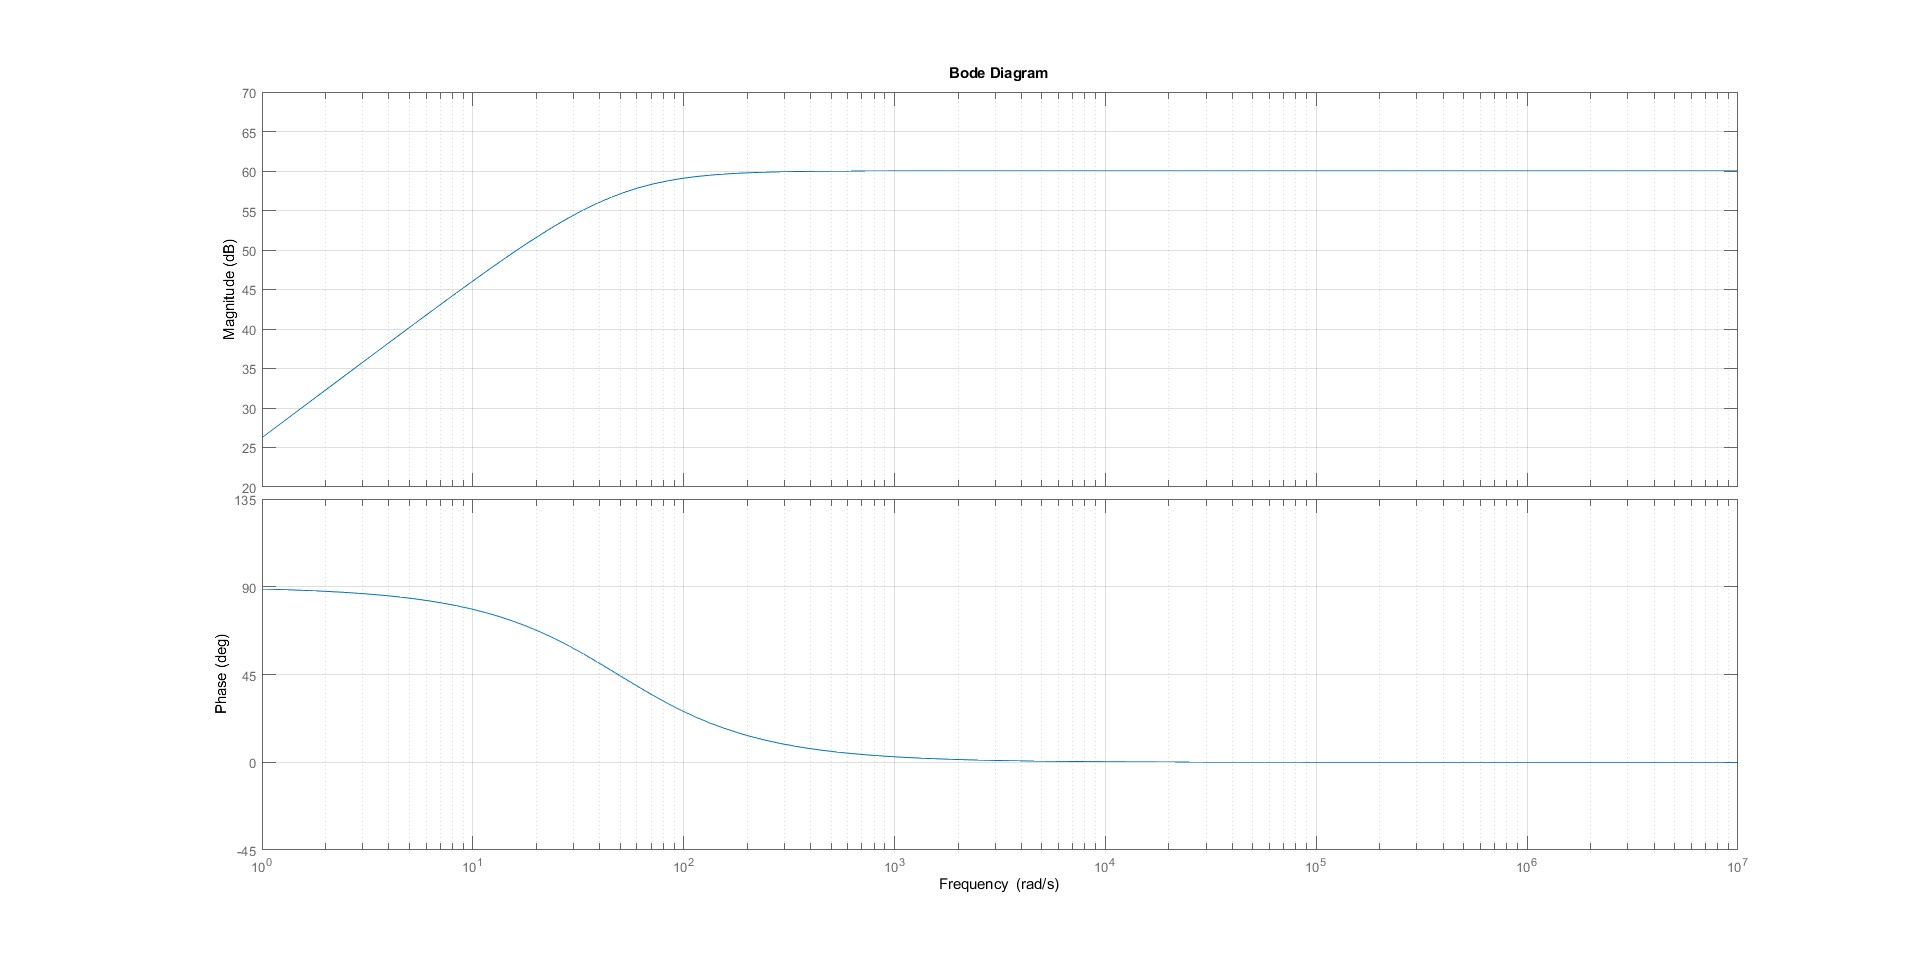
\includegraphics[width=1\textwidth]{Figure/BodeAnalitico.jpg}
    \caption{Diagramma di Bode ottenuto dall'analisi analitica}
    \label{fig:bodeAnalitico}
\end{figure}
\newpage
\subsection{Simulazione SPICE}\label{subsec:simulazione_spice}
Simulando su SPICE il circuito otteniamo il seguente diagramma di Bode.\\
\begin{figure}[h]
    \centering
    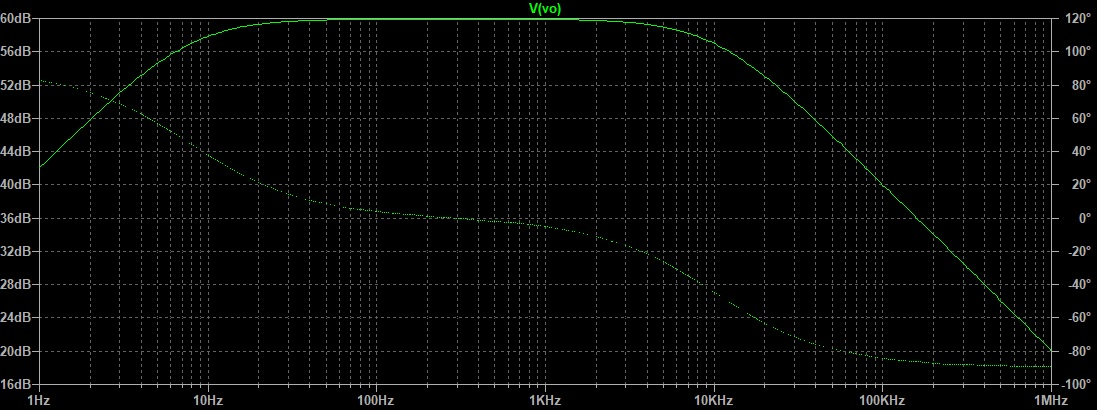
\includegraphics[width=1\textwidth]{Figure/Bode 1.4_1.jpg}
    \caption{Grafico di Bode non ideale}
    \label{fig:bode_non_ideale}
\end{figure}\\
Il precedente diagramma differisce da quello calcolato, in quanto l'amplificatore operazionale utilizzato da SPICE non è un amplificatore ideale.\\
Per avere condizioni simili a quelle di un amplificatore ideale dobbiamo incrementare il rapporto guadagno x larghezza di banda. Dopo aver incrementato il rapporto di un fattore 1000 infatti la simulazione produce il seguente grafico.\\
\begin{figure}[h]
    \centering
    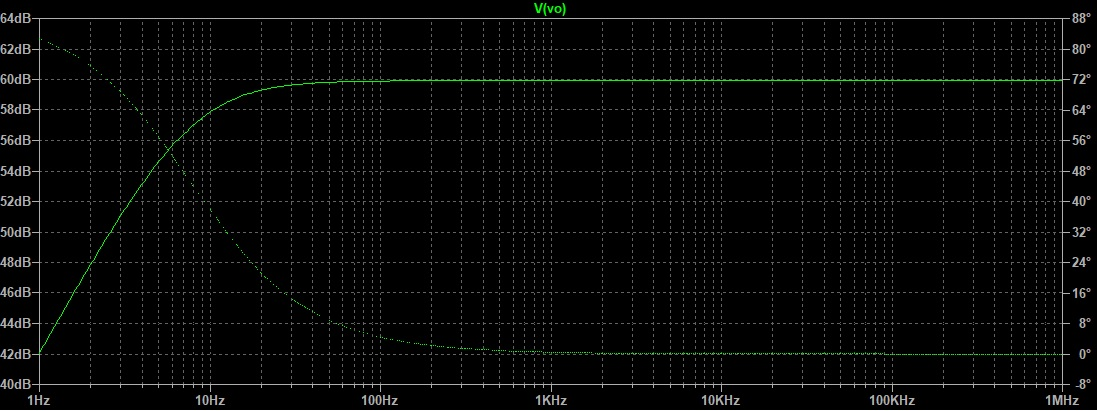
\includegraphics[width=1\textwidth]{Figure/Bode 1.4_2.jpg}
    \caption{Grafico di Bode ideale}
    \label{fig:bode_ideale}
\end{figure}\\

\subsection{Aumentare la Banda}\label{subsec:aumentare_banda}
Per aumentare la banda dell'amplificatore potremmo ridurre il guadagno.

\newpage
\subsection{Simulazione SPICE per Amplificatore LT1115}\label{subsec:simulazione_LT1115}
Si considera ora una variante del circuito, sostituendo l'amplificatore operazionale ideale con un amplificatore reale LT1115.
\begin{figure}[h]
    \centering
    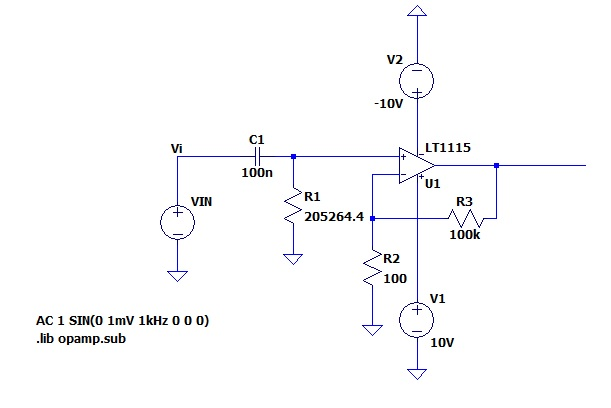
\includegraphics[width=0.9\textwidth]{Figure/Circuito.jpg}
    \caption{Variante circuito del primo esercizio}
    \label{fig:Circuito}
\end{figure}\\
Listato SPICE della rete considerata:\\
\\
C1 N002 Vi 100n\\
R1 N002 0 205264.4\\
R2 N004 0 100\\
R3 N003 N004 100k\\
V1 N005 0 10V\\
V2 N001 0 -10V\\
VIN Vi 0 AC 1 SIN(0 1mV 1kHz 0 0 0)\\
XU1 N002 N004 N005 N001 N003 LT1115\\
.tran 5m\\
.lib opamp.sub\\
.lib LTC.lib\\
.backanno\\
.end\\
\\
Alimentando il circuito con un generatore di tensione sinusoidale con ampiezza 1 mV e frequenza 1 KHz si ottiene la seguente forma d'onda in uscita dall'amplificatore.
\newpage
\begin{figure}[h]
    \centering
    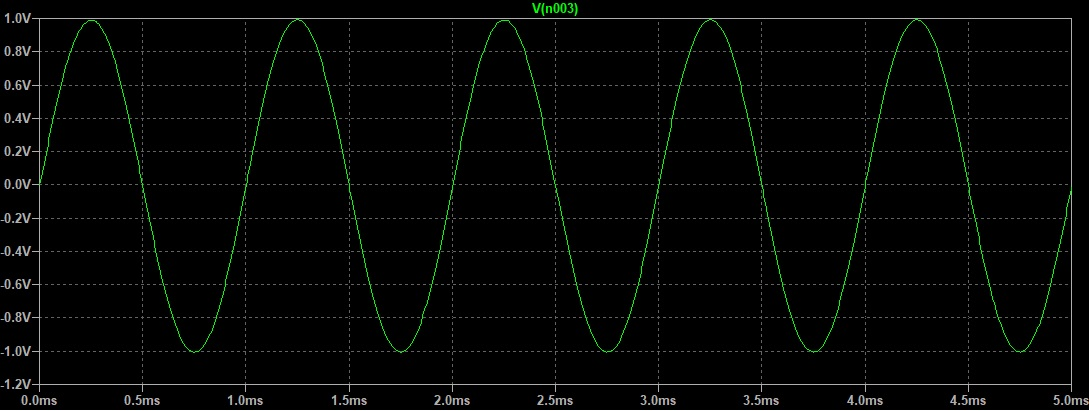
\includegraphics[width=1\textwidth]{Figure/Uscita 1.6.jpg}
    \caption{Forma d'onda in uscita dall'amplificatore per parametri di 1 mV e 1 KHz}
    \label{fig:UscitaCircuito}
\end{figure}

\subsection{Diagramma di Bode}\label{subsec:diagramma_bode_variante}
Simulando con SPICE il circuito per frequenze da 1 Hz a 1 MHz si ottiene il seguente diagramma di Bode.
\begin{figure}[h]
    \centering
    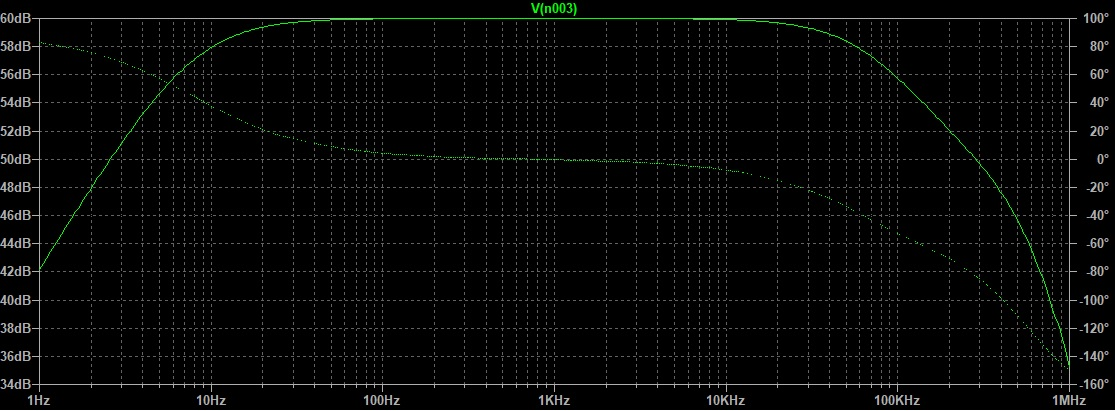
\includegraphics[width=1\textwidth]{Figure/Bode 1.7.jpg}
    \caption{Grafico di Bode per amplificatore LT1115 da 1 Hz a 1 MHz}
    \label{fig:bode_lt1115}
\end{figure}

\newpage
\subsection{Tensione di Saturazione}\label{subsec:saturazione}
Simulando varie ampiezze di ingresso con SPICE otteniamo il seguente risultato\\
\begin{figure}[h]
    \centering
    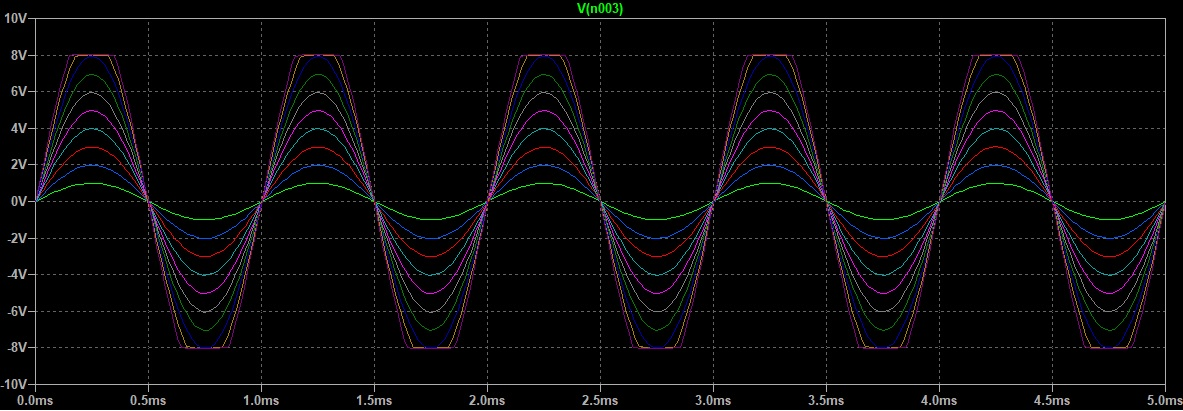
\includegraphics[width=1\textwidth]{Figure/SaturazioneAnalisi 1.8.1.jpg}
    \caption{Forme d'onda in uscita per varie ampiezze in ingresso}
    \label{fig:saturazione_analisi}
\end{figure}\\
Osservando il grafico possiamo notare che la tensione di saturazione per l'amplificatore LT1115 è di 8 V
\newline
Fissiamo ora la frequenza del generatore a 1KHz e calcoliamo analiticamente l'ampiezza di ingresso per la quale l'amplificatore satura.\\
$$s = j\omega$$ $$\omega = 2\pi * f$$
\begin{equation}\label{eq:eqAmpiezzaSaturazione}
V_{o} = V_{i}\dfrac{\dfrac{j\omega R_{2}C_{2}(R_{3}+R_{4})}{R_{3}}}{1+j\omega C_{2}R_{2}} = V_{i}\dfrac{j\omega20,55}{1 + j\omega0,0205} = V_{i}\dfrac{j441100\pi}{1 + j41\pi}
\end{equation}
\begin{equation}\label{eq:eqAmpiezzaSaturazioneModuli}
|V_{o}| = |V_{i}| * \big| \dfrac{j441100\pi}{1 + j41\pi} \big|
\end{equation}
\begin{equation}\label{eq:eqAmpiezzaSaturazioneRisultato}
|V_{i}| < \dfrac{8}{1002,39} = 8\hspace{2pt}mV
\end{equation}
Come trovato nell'equazione \ref{eq:eqAmpiezzaSaturazioneRisultato} l'ampiezza in ingresso per la quale l'amplificatore satura è 8 mV.\\
Simulando ora il circuito con un'ampiezza di ingresso di 16 mV otteniamo il seguente risultato
\begin{figure}[h]
    \centering
    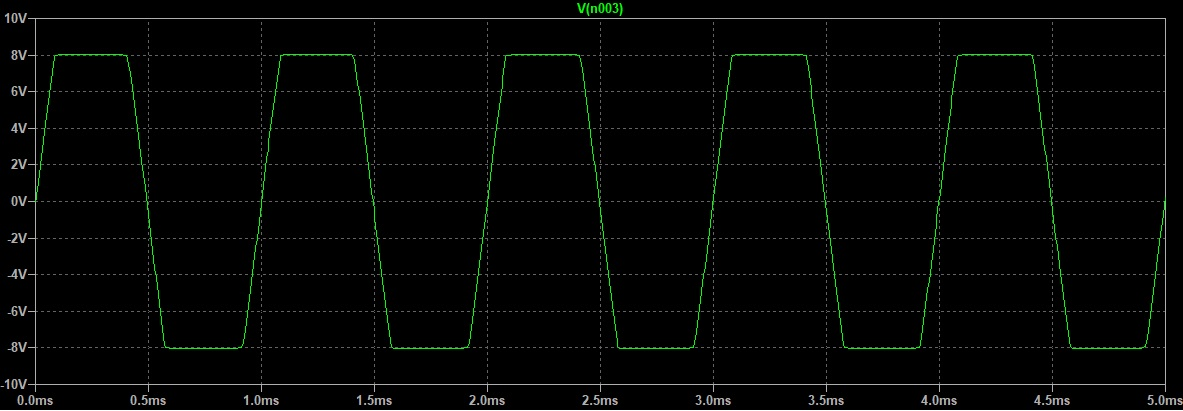
\includegraphics[width=1\textwidth]{Figure/SaturazioneUscita 1.8.2.jpg}
    \caption{Forme d'onda in uscita per un ampiezza di 16 mV}
    \label{fig:saturazione_uscita}
\end{figure}\\